\documentclass{article}

% Language setting
\usepackage[english]{babel}

\usepackage[a4paper,top=2cm,bottom=2cm,left=3cm,right=3cm,marginparwidth=1.75cm]{geometry}

% Useful packages
\usepackage{amsmath}
\usepackage{graphicx}
\usepackage{listings}
\usepackage[colorlinks=true, allcolors=blue]{hyperref}

\title{Homework 01\\"OpenSSL support to GCM"}
\author{Andrea Panceri 1884749}

\begin{document}
\maketitle

\section{Introduction to OpenSSL}

OpenSSL is an open-source command line tool, it is used for various purposes connected with cryptography like create private key,install TLS(or SSL) certificate, performing encryption/decryption, etc. OpenSSL is licensed under an Apache-style license, which fundamentally implies that you are free to get and use it for business and non-business purposes subject to some basic permit conditions, for this reason many web servers use it. The most recent version is the 3.0 series supported until 7th September 2026. This is also a Long Term Support (LTS) version.\\For other information this is the official website: \href{https://www.openssl.org/}{OpenSSL website}

\section{Forks of OpenSSL}

Before starting, let's give a simple explanation of what a fork is. In software engineering, a project fork happens when developers take a duplicate of source code from one software package and start independent development on it, creating a distinct and separate piece of software. The term often implies not merely a development branch, but also a split in the developer community. Grounds for forking are varying user preferences or discontinued development of the original software.\\Free and open-source software,like OpenSSL, is that which, by definition, may be forked from the original development team without prior permission, and without violating copyright law.\\As you can imagine OpenSSL has several forks, now let's talk about the most famous that can be found online.\\\\
The most famous fork of OpenSSL is certainly libreSSL, it is a version of the TLS/crypto stack forked from OpenSSL in 2014 in response to the Heartbleed security vulnerability, with goals of modernizing the codebase, improving security, and applying best practice development processes. From the official \href{https://www.libressl.org/}{website} we can read the goal of the project:\\
\begin{itemize}
\item Modernize the OpenSSL codebase to make it easier to audit, understand and repair.
\item Apply best-practice development processes:
\begin{itemize}
\item Code Review
\item Frequent releases.
\item Open development process.
\end{itemize}
\item Remove obsolete or broken features and operating system support.
\item Use and encourage the incorporation of secure programming interfaces in operating systems.
\item Provide secure alternatives on operating systems that do not yet have secure programming interfaces available.
\end{itemize}
it is very supported and in fact it can be seen that the latest stable release is 3.6.0 that is dated October 5th, 2022. In addition it work well on the following platforms: Linux, FreeBSD, NetBSD, HP-UX, Solaris, macOS and AIX.\\\\
BoringSSL is another fork of OpenSSL that is designed to meet Google's needs.it is an open source project, it is not intended for general use, as OpenSSL is. it isn't recommend that third parties depend upon it. BoringSSL arose because Google used OpenSSL for many years in various ways and, over time, built up a large number of patches that were maintained while tracking upstream OpenSSL. As Google's product portfolio became more complex, more copies of OpenSSL sprung up and the effort involved in maintaining all these patches in multiple places was growing steadily.Currently BoringSSL is the SSL library in Chrome/Chromium, Android and a number of other apps/programs. The community that follows its development is very active, in fact from the  \href{https://github.com/google/boringssl}{github codebase} you can see how frequent updates are.\\\\
The Agglomerated SSL was made in 2009 by Marco Peereboom (an OpenSSL developer). It doesn’t change the encryption code itself. Instead, it simplifies the interface. This makes Agglomerated SSL easier to include in different programs. It is used, for example, to allow VLC to be able to play Blu-ray discs. It is not longer support ,on the repository we can see the last change is on 25 August 2015.\\\\
The \href{https://github.com/open-quantum-safe/openssl/tree/OQS-OpenSSL_1_1_1-stable}{Open Quantum Safe OpenSSL repository} contains a fork of OpenSSL 1.1.1 that adds quantum-resistant key exchange and signature algorithms using liboqs for prototyping purposes. The library supports both hybrid and post-quantum key exchange and authentication. It is co-developed by Microsoft and is born for prototyping, experimentation, and for evaluating quantum-resistant cryptography. Post-quantum cryptography is an active area of research, and the security of proposed quantum-resistant algorithms may rapidly change as research advances. This fork is at an experimental stage, and has not received the same level of auditing and analysis that OpenSSL has received, the last commit on the repository is dated 29 august 2022.\\
These are all the forks that I was able to find online and above all that are continuously supported, certainly the first two mentioned as well as having a large community and are extremely used.


\section{How to use AES with GCM}

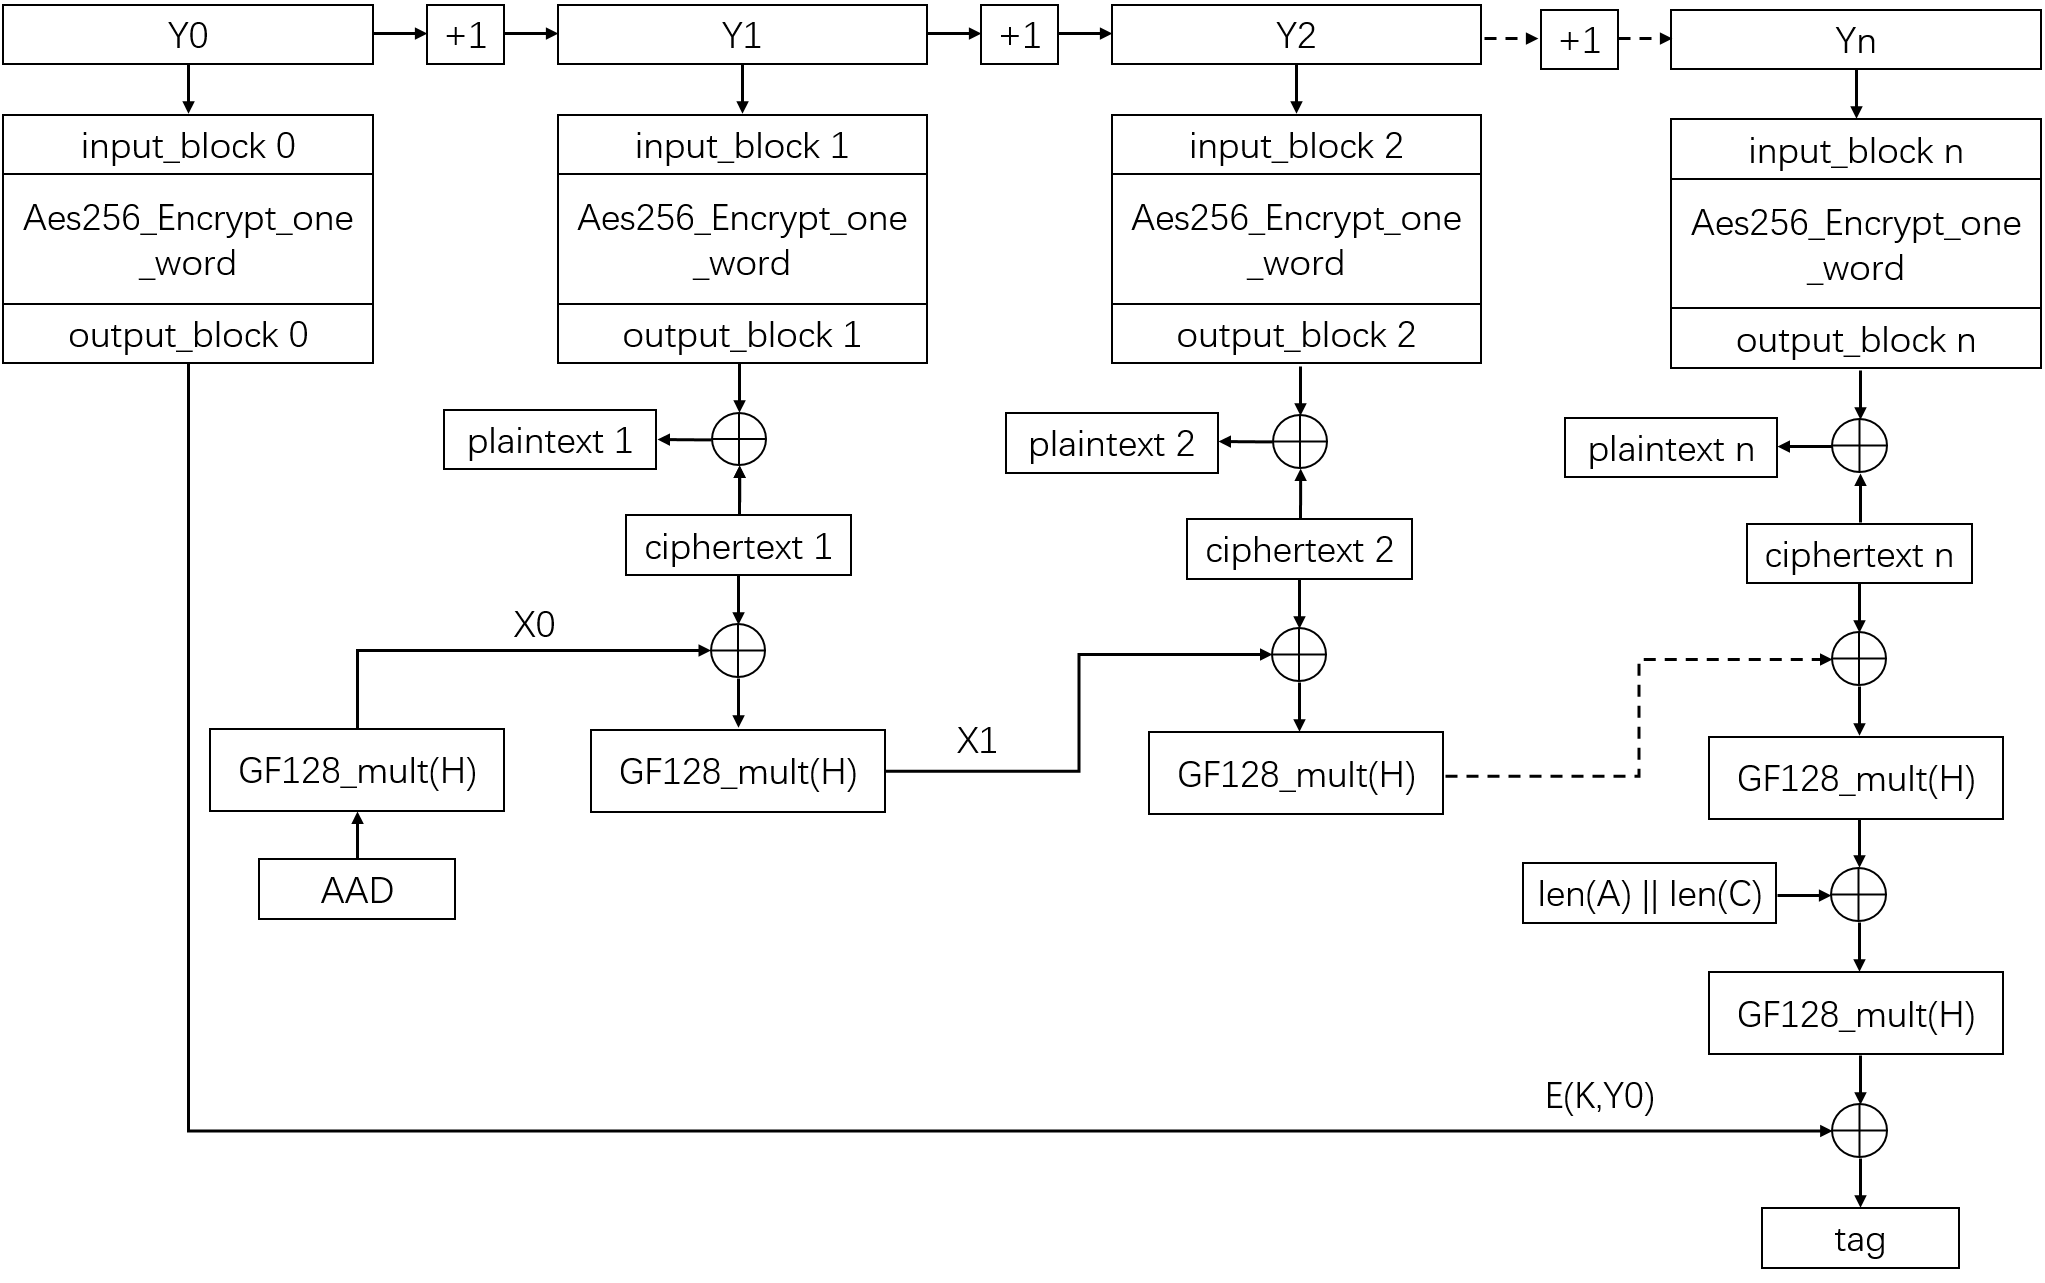
\includegraphics[width=\textwidth]{hw01-1884749.png}
\href{https://www.nist.gov/publications/advanced-encryption-standard-aes}{The Advanced Encryption Standard (AES)} is a specification for the encryption of electronic data established by NIST(National Institute of Standards and Technology) in 2001.The algorithm described by AES is a symmetric-key algorithm, meaning the same key is used for both encrypting and decrypting the data. It applying multiple rounds to encrypt data, these encryption rounds are the reason behind the impenetrability of AES, as there are far too many rounds to break through. There are three lengths of AES encryption keys. Each key length has a different number of possible key combinations: 128-bit, 192-bit and 256-bit key length. Even though the key length of this encryption method varies, its block size - 128-bits stays fixed. The most used today is 256-bit AES encryption.\\
\href{https://nvlpubs.nist.gov/nistpubs/legacy/sp/nistspecialpublication800-38d.pdf}{GCM(Galois/Counter Mode)} is a mode of operation for symmetric-key cryptographic block ciphers. The operation is an authenticated encryption algorithm designed to provide both data authenticity (integrity) and confidentiality. GCM is defined for block ciphers with a block size of 128 bits. it can accept initialization vectors of arbitrary length. Different block cipher modes of operation can have significantly different performance and efficiency characteristics, even when used with the same block cipher. Today GCM is the most used, in combination with AES.\\\\
From the old documentation we can read that OpenSSL supports the ability to perform authenticated encryption and decryption, but unfortunately enc command does not support authenticated encryption modes like GCM, and will not support such modes in the future. This is due to having to begin streaming output before the authentication tag could be validated. When this command is used in a pipeline, the receiving end will not be able to roll back upon authentication failure. The AEAD modes currently in common use also suffer from catastrophic failure of confidentiality and/or integrity upon reuse of key/iv/nonce, and since openssl enc places the entire burden of key/iv/nonce management upon the user, the risk of exposing AEAD modes is too great to allow (More detail in the \href{https://www.openssl.org/docs/manmaster/man1/openssl-enc.html}{official documentation}).\\
Instead, from the latest versions it is possible to use the enc command with aes-256-gcm. Now we show examples of how it is possible to encrypt and decrypt a file on Ubuntu using libreSSL:
\begin{lstlisting}
openssl version --> libreSSL 3.6.0

ENCRYPTION:
openssl aes-256-gcm -in esempio -out esempioenc.txt
enter aes-256-gcm encryption password: (any password)
verifying -enter aes-256-gcm encryption password: (same password)

DECRYPTION:
openssl aes-256-gcm -d -in esempioenc.txt -out esempiodec.txt
enter aes-256-gcm encryption password: (same password of encryption)
bad decrypt
\end{lstlisting}
Moreover these commands are almost identical in OpenSSL, so it is possible to do everything that has been shown.\\Unfortunately neither with OpenSSL nor with other forks is it possible to check the integrity through command line commands, most likely related to the inherent facts on security reported in the previous documentation, we can notice the bad decrypt in result, that meaning a problem in the check of integrity. So if we want to do an integrity check we have to use a different method, we have to create programs.
OpenSSL supports aes-256-gcm as an algorithm.You can use the \href{https://wiki.openssl.org/index.php/EVP_Authenticated_Encryption_and_Decryption}{EVP interface} to call aes-256-gcm algorithm,this library within OpenSSL provides functions for performing symmetric encryption and decryption operations across a wide range of algorithms and modes. As with standard symmetric encryption you will need to know the following:
\begin{itemize}
\item Algorithm (currently only AES is supported).
\item Mode (currently only GCM and CCM are supported).
\item Key.
\item Initialisation Vector (IV).
\end{itemize}
In addition you can (optionally) provide some Additional Authenticated Data (AAD). The AAD data is not encrypted, and is typically passed to the recipient in plaintext along with the ciphertext. An example of AAD is the IP address and port number in a IP header used with IPsec.\\
We now show, reporting the official documentation, examples of authenticated encryption and decryption in c programming language that make use of aes and gcm, in this way we can achieve the check of integrity.\\

\subsection{Authenticated Encryption using GCM mode}
Encryption is performed in much the same way as for symmetric encryption. The main differences are:
\begin{itemize}
\item You may optionally pass through an IV length using EVP\_CIPHER\_CTX\_ctrl.
\item AAD data is passed through in zero or more calls to EVP\_EncryptUpdate, with the output buffer set to NULL.
\item Once private data has been added using EVP\_EncryptUpdate (non-NULL output buffer), you cannot add AAD data.
\item After the EVP\_EncryptFinal\_ex call a new call to EVP\_CIPHER\_CTX\_ctrl retrieves the tag.
\end{itemize}
See the code below for an example:

\begin{lstlisting}
int gcm_encrypt(unsigned char *plaintext, int plaintext_len,
                unsigned char *aad, int aad_len,
                unsigned char *key,
                unsigned char *iv, int iv_len,
                unsigned char *ciphertext,
                unsigned char *tag)
{
    EVP_CIPHER_CTX *ctx;

    int len;

    int ciphertext_len;


    /* Create and initialise the context */
    if(!(ctx = EVP_CIPHER_CTX_new()))
        handleErrors();

    /* Initialise the encryption operation. */
    if(1 != EVP_EncryptInit_ex(ctx, EVP_aes_256_gcm(), NULL, NULL, NULL))
        handleErrors();

    /*
     * Set IV length if default 12 bytes (96 bits) is not appropriate
     */
    if(1 != EVP_CIPHER_CTX_ctrl(ctx, EVP_CTRL_GCM_SET_IVLEN, iv_len, NULL))
        handleErrors();

    /* Initialise key and IV */
    if(1 != EVP_EncryptInit_ex(ctx, NULL, NULL, key, iv))
        handleErrors();

    /*
     * Provide any AAD data. This can be called zero or more times as
     * required
     */
    if(1 != EVP_EncryptUpdate(ctx, NULL, &len, aad, aad_len))
        handleErrors();

    /*
     * Provide the message to be encrypted, and obtain the encrypted output.
     * EVP_EncryptUpdate can be called multiple times if necessary
     */
    if(1 != EVP_EncryptUpdate(ctx, ciphertext, &len, plaintext, plaintext_len))
        handleErrors();
    ciphertext_len = len;

    /*
     * Finalise the encryption. Normally ciphertext bytes may be written at
     * this stage, but this does not occur in GCM mode
     */
    if(1 != EVP_EncryptFinal_ex(ctx, ciphertext + len, &len))
        handleErrors();
    ciphertext_len += len;

    /* Get the tag */
    if(1 != EVP_CIPHER_CTX_ctrl(ctx, EVP_CTRL_GCM_GET_TAG, 16, tag))
        handleErrors();

    /* Clean up */
    EVP_CIPHER_CTX_free(ctx);

    return ciphertext_len;
}
\end{lstlisting}
\subsection{Authenticated Decryption using GCM mode}
Again, the decryption operation is much the same as for normal symmetric decryption. The main differences are:
\begin{itemize}
\item You may optionally pass through an IV length using EVP\_CIPHER\_CTX\_ctrl.
\item AAD data is passed through in zero or more calls to EVP\_DecryptUpdate, with the output buffer set to NULL.
\item Prior to the EVP\_DecryptFinal\_ex call a new call to EVP\_CIPHER\_CTX\_ctrl provides the tag.
\item A non positive return value from EVP\_DecryptFinal\_ex should be considered as a failure to authenticate ciphertext and/or AAD. It does not necessarily indicate a more serious error..
\end{itemize}

See the code example below:
\begin{lstlisting}
int gcm_decrypt(unsigned char *ciphertext, int ciphertext_len,
                unsigned char *aad, int aad_len,
                unsigned char *tag,
                unsigned char *key,
                unsigned char *iv, int iv_len,
                unsigned char *plaintext)
{
    EVP_CIPHER_CTX *ctx;
    int len;
    int plaintext_len;
    int ret;

    /* Create and initialise the context */
    if(!(ctx = EVP_CIPHER_CTX_new()))
        handleErrors();

    /* Initialise the decryption operation. */
    if(!EVP_DecryptInit_ex(ctx, EVP_aes_256_gcm(), NULL, NULL, NULL))
        handleErrors();

    /* Set IV length. Not necessary if this is 12 bytes (96 bits) */
    if(!EVP_CIPHER_CTX_ctrl(ctx, EVP_CTRL_GCM_SET_IVLEN, iv_len, NULL))
        handleErrors();

    /* Initialise key and IV */
    if(!EVP_DecryptInit_ex(ctx, NULL, NULL, key, iv))
        handleErrors();

    /*
     * Provide any AAD data. This can be called zero or more times as
     * required
     */
    if(!EVP_DecryptUpdate(ctx, NULL, &len, aad, aad_len))
        handleErrors();

    /*
     * Provide the message to be decrypted, and obtain the plaintext output.
     * EVP_DecryptUpdate can be called multiple times if necessary
     */
    if(!EVP_DecryptUpdate(ctx, plaintext, &len, ciphertext, ciphertext_len))
        handleErrors();
    plaintext_len = len;

    /* Set expected tag value. Works in OpenSSL 1.0.1d and later */
    if(!EVP_CIPHER_CTX_ctrl(ctx, EVP_CTRL_GCM_SET_TAG, 16, tag))
        handleErrors();

    /*
     * Finalise the decryption. A positive return value indicates success,
     * anything else is a failure - the plaintext is not trustworthy.
     */
    ret = EVP_DecryptFinal_ex(ctx, plaintext + len, &len);

    /* Clean up */
    EVP_CIPHER_CTX_free(ctx);

    if(ret > 0) {
        /* Success */
        plaintext_len += len;
        return plaintext_len;
    } else {
        /* Verify failed */
        return -1;
    }
}
\end{lstlisting}
These codes just shown are to be integrated in a C file, in main all the necessary variables in the function signature must be initialized, including all the openSSL libraries (which can be found from the official site) and then simply launch the functions and manage the results.

\end{document}